\documentclass{standalone}
\usepackage[calc]{picture}
\usepackage{graphicx,transparent,color,amsmath,amssymb,amsfonts,tikz}
\graphicspath{Fig_SIM_subfigs}
\setlength{\unitlength}{1in}

\usepackage{helvet}
\renewcommand{\familydefault}{\sfdefault}
\begin{document}


\begin{picture}(4.5, 4.8)(-0.15,-15.9)
\put(-0.1,-16){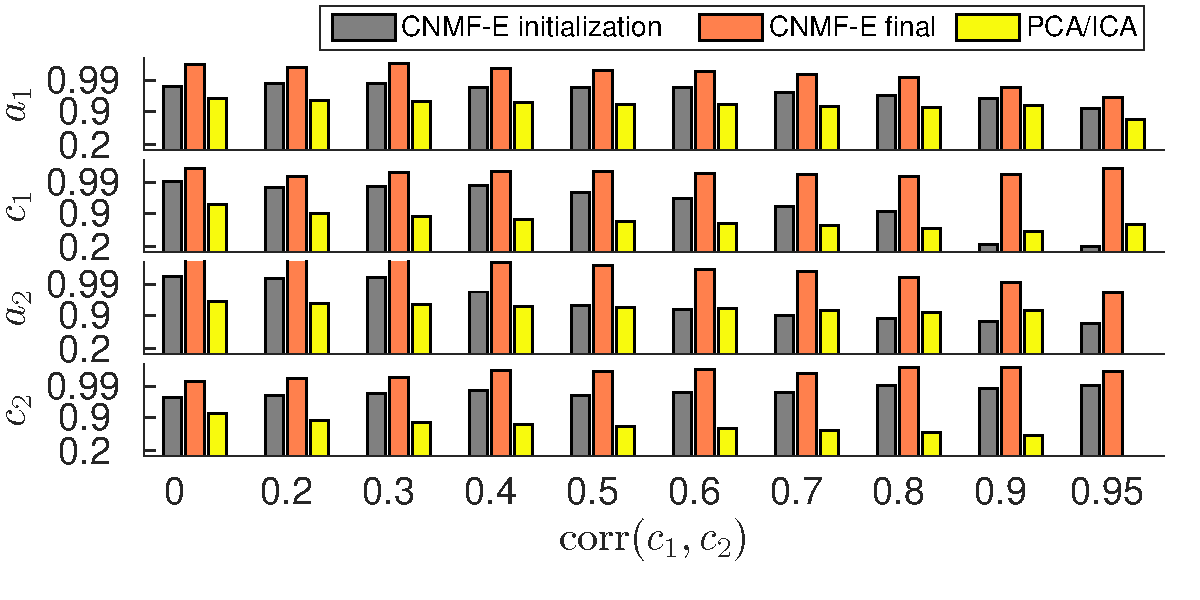
\includegraphics[height=2.2in]{Fig_SIM_subfigs/similarity_corr.pdf}}
\put(-0.1, -13.7){\Large\textbf{B}}
\put(1.55, -13.65){Extraction accuracy}

\put(0.7,-13.5){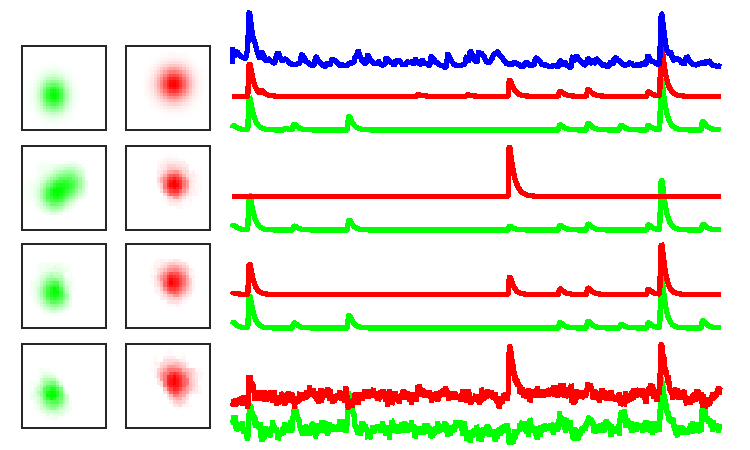
\includegraphics[height=2.2in]{Fig_SIM_subfigs/example_corr.pdf}}
\put(-0.1, -11.35){\Large\textbf{A}}
\put(1.55, -11.3){Example simulation}
% \put(3.4, -3.65){\textbf{I}}
\put(-0, -11.75){ground truth}
\put(0, -12.19){CNMF-E}
\put(0, -12.32){initialization}
\put(0, -12.66){CNMF-E}
\put(0, -12.79){final}
\put(0, -13.2){PCA/ICA}

% \put(4.5, -3.65){\footnotesize Example simulation}

\end{picture}
\end{document}
